% GENERATED by make_schematic_tex.py -- edit the script, not this file.
\documentclass[tikz,border=4pt]{standalone}
\usepackage[T1]{fontenc}
\usepackage{lmodern}
\usetikzlibrary{arrows.meta}
\definecolor{cthin}{HTML}{6A5ACD}
\definecolor{cthick}{HTML}{8BB174}
\definecolor{cpink}{HTML}{EB078E}
\definecolor{ccrust}{RGB}{222,222,222}
\definecolor{cmantle}{RGB}{252,226,204}
\definecolor{cslab}{RGB}{128,138,152}
\definecolor{cwater}{RGB}{198,224,240}
\definecolor{cmagma}{RGB}{236,112,52}
\definecolor{txt}{RGB}{85,85,85}
\begin{document}
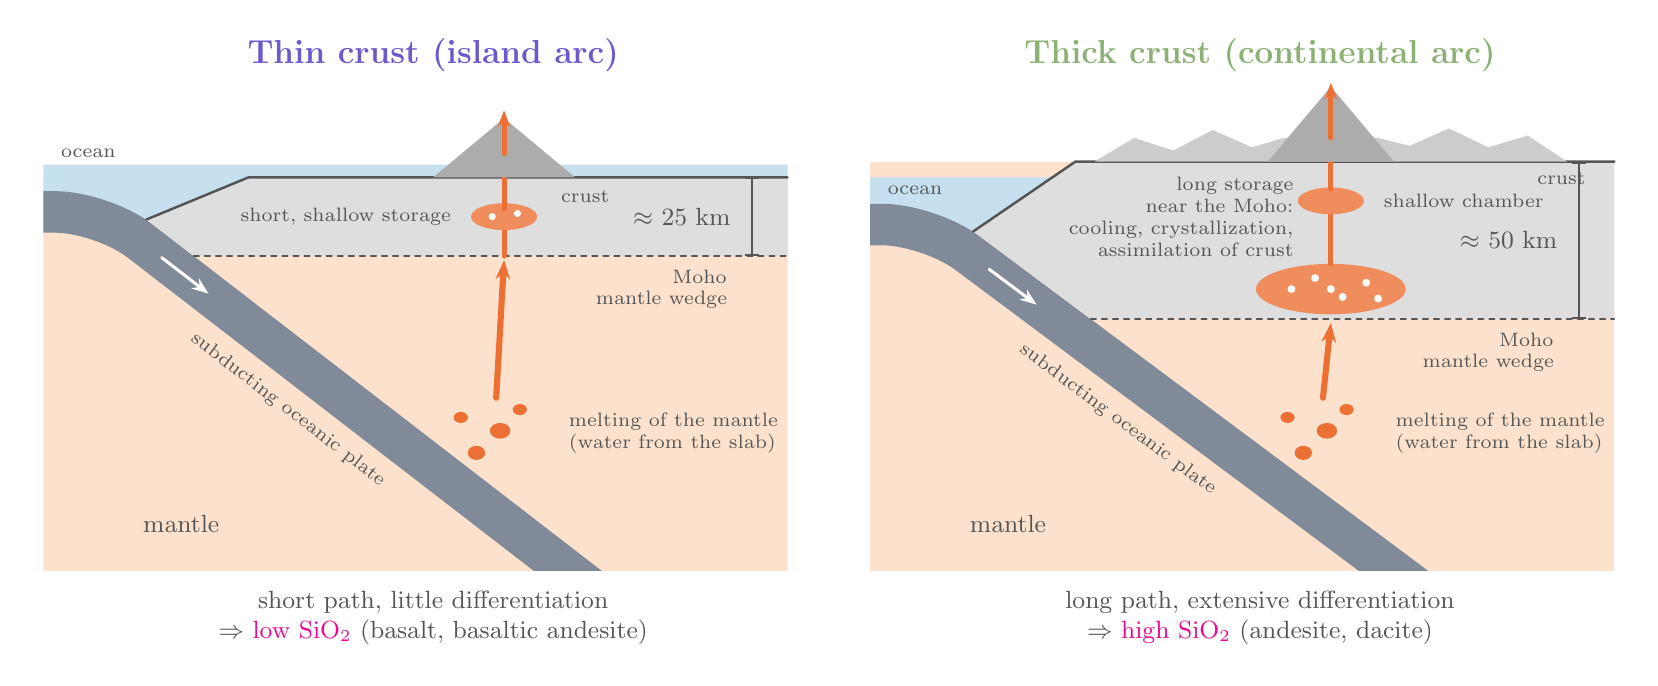
\begin{tikzpicture}[x=1cm,y=1cm,line cap=round,line join=round]
\useasboundingbox (-0.65,-1.1) rectangle (19.7,6.9);
\begin{scope}[shift={(0.00,0)}]
\begin{scope}
\clip (-0.45,0) rectangle (9.00,6.30);
\fill[cmantle] (-0.45,0) rectangle (9.00,5.00);
\fill[cwater] (-0.450,5.160) -- (9.000,5.160) -- (9.000,5.000) -- (2.157,5.000) -- (0.857,4.463) -- (0.696,4.255) -- (0.300,4.560) -- (-0.450,4.560) -- cycle;
\draw[cslab, line width=15pt, line cap=butt, rounded corners=0.6cm] (-0.75,4.56) -- (0.30,4.56) -- (6.60,-0.30);
\fill[ccrust] (0.857,4.463) -- (2.157,5.000) -- (9.000,5.000) -- (9.000,4.000) -- (1.457,4.000) -- cycle;
\end{scope}
\draw[txt, line width=0.9pt] (0.857,4.463) -- (2.157,5.000) -- (9.000,5.000);
\draw[txt, line width=0.5pt, dash pattern=on 2pt off 2pt] (1.457,4.00) -- (9.00,4.00);
\node[txt, font=\scriptsize, anchor=north east] at (8.35,3.95) {Moho};
\draw[white, line width=1.1pt, -{Stealth[length=6pt]}] (1.052,3.980) -- (1.646,3.522);
\node[txt, font=\scriptsize, rotate=-37.6] at (2.656,2.048) {subducting oceanic plate};
\fill[cmagma] (5.05,1.50) ellipse (0.11 and 0.09);
\fill[cmagma] (5.35,1.78) ellipse (0.13 and 0.10);
\fill[cmagma] (4.85,1.95) ellipse (0.09 and 0.07);
\fill[cmagma] (5.60,2.05) ellipse (0.09 and 0.07);
\node[txt, font=\scriptsize, anchor=west, align=left] at (6.1,1.75) {melting of the mantle\\(water from the slab)};
\node[txt, font=\scriptsize] at (7.4,3.45) {mantle wedge};
\draw[cmagma, line width=2.2pt, -{Stealth[length=7pt]}] (5.3,2.2) -- (5.40,3.95);
\draw[cmagma, line width=1.8pt] (5.40,4.00) -- (5.40,4.50);
\fill[cmagma!80!white] (5.40,4.50) ellipse (0.42 and 0.17);
\fill[white] (5.25,4.50) circle (0.045); \fill[white] (5.57,4.54) circle (0.045);
\draw[cmagma, line width=1.8pt] (5.40,4.60) -- (5.40,5.60);
\node[txt, font=\scriptsize, anchor=east] at (4.85,4.50) {short, shallow storage};
\fill[gray!65] (4.5,5.00) -- (5.4,5.75) -- (6.3,5.00) -- cycle;
\draw[cmagma, line width=1.8pt, -{Stealth[length=6pt]}] (5.40,5.30) -- (5.40,5.85);
\draw[txt, {Bar[width=5pt]}-{Bar[width=5pt]}, line width=0.8pt] (8.55,4.00) -- (8.55,5.00);
\node[txt, font=\small, anchor=east] at (8.4,4.50) {$\approx$ 25 km};
\node[txt, font=\scriptsize, anchor=west] at (6.00,4.75) {crust};
\node[txt, font=\small] at (1.3,0.6) {mantle};
\node[txt, font=\scriptsize, anchor=west] at (-0.35,5.30) {ocean};
\node[cthin, font=\large\bfseries] at (4.5,6.55) {Thin crust (island arc)};
\node[txt, font=\small, align=center] at (4.5,-0.6) {short path, little differentiation\\ $\Rightarrow$ {\color{cpink}low SiO$_2$} (basalt, basaltic andesite)};
\end{scope}
\begin{scope}[shift={(10.50,0)}]
\begin{scope}
\clip (-0.45,0) rectangle (9.00,6.50);
\fill[cmantle] (-0.45,0) rectangle (9.00,5.20);
\fill[cwater] (-0.450,5.000) -- (1.865,5.000) -- (0.858,4.312) -- (0.701,4.101) -- (0.300,4.400) -- (-0.450,4.400) -- cycle;
\draw[cslab, line width=15pt, line cap=butt, rounded corners=0.6cm] (-0.75,4.40) -- (0.30,4.40) -- (6.60,-0.30);
\fill[ccrust] (0.858,4.312) -- (2.158,5.200) -- (9.000,5.200) -- (9.000,3.200) -- (2.349,3.200) -- cycle;
\end{scope}
\draw[txt, line width=0.9pt] (0.858,4.312) -- (2.158,5.200) -- (9.000,5.200);
\draw[txt, line width=0.5pt, dash pattern=on 2pt off 2pt] (2.349,3.20) -- (9.00,3.20);
\node[txt, font=\scriptsize, anchor=north east] at (8.35,3.15) {Moho};
\draw[white, line width=1.1pt, -{Stealth[length=6pt]}] (1.061,3.832) -- (1.663,3.383);
\node[txt, font=\scriptsize, rotate=-36.7] at (2.696,1.926) {subducting oceanic plate};
\fill[cmagma] (5.05,1.50) ellipse (0.11 and 0.09);
\fill[cmagma] (5.35,1.78) ellipse (0.13 and 0.10);
\fill[cmagma] (4.85,1.95) ellipse (0.09 and 0.07);
\fill[cmagma] (5.60,2.05) ellipse (0.09 and 0.07);
\node[txt, font=\scriptsize, anchor=west, align=left] at (6.1,1.75) {melting of the mantle\\(water from the slab)};
\node[txt, font=\scriptsize] at (7.4,2.65) {mantle wedge};
\draw[cmagma, line width=2.2pt, -{Stealth[length=7pt]}] (5.3,2.2) -- (5.40,3.15);
\fill[cmagma!80!white] (5.40,3.58) ellipse (0.95 and 0.32);
\fill[white] (4.90,3.58) circle (0.05);
\fill[white] (5.20,3.72) circle (0.05);
\fill[white] (5.55,3.48) circle (0.05);
\fill[white] (5.85,3.66) circle (0.05);
\fill[white] (5.40,3.58) circle (0.05);
\fill[white] (6.00,3.46) circle (0.05);
\draw[cmagma, line width=1.8pt] (5.40,3.90) -- (5.40,4.65);
\fill[cmagma!80!white] (5.40,4.70) ellipse (0.42 and 0.17);
\draw[cmagma, line width=1.8pt] (5.40,4.85) -- (5.40,5.90);
\node[txt, font=\scriptsize, anchor=east, align=right] at (5.05,4.50) {long storage\\near the Moho:\\cooling, crystallization,\\assimilation of crust};
\node[txt, font=\scriptsize, anchor=west] at (5.95,4.70) {shallow chamber};
\fill[gray!40] (2.40,5.20) -- (2.90,5.50) -- (3.40,5.34) -- (3.90,5.60) -- (4.40,5.38) -- (4.80,5.50) -- (6.00,5.50) -- (6.40,5.40) -- (6.90,5.62) -- (7.40,5.38) -- (7.90,5.53) -- (8.40,5.20) -- cycle;
\fill[gray!65] (4.6,5.20) -- (5.4,6.15) -- (6.2,5.20) -- cycle;
\draw[cmagma, line width=1.8pt, -{Stealth[length=6pt]}] (5.40,5.50) -- (5.40,6.20);
\draw[txt, {Bar[width=5pt]}-{Bar[width=5pt]}, line width=0.8pt] (8.55,3.20) -- (8.55,5.20);
\node[txt, font=\small, anchor=east] at (8.4,4.20) {$\approx$ 50 km};
\node[txt, font=\scriptsize, anchor=west] at (7.90,4.98) {crust};
\node[txt, font=\small] at (1.3,0.6) {mantle};
\node[txt, font=\scriptsize, anchor=west] at (-0.35,4.83) {ocean};
\node[cthick, font=\large\bfseries] at (4.5,6.55) {Thick crust (continental arc)};
\node[txt, font=\small, align=center] at (4.5,-0.6) {long path, extensive differentiation\\ $\Rightarrow$ {\color{cpink}high SiO$_2$} (andesite, dacite)};
\end{scope}
\end{tikzpicture}
\end{document}
